\documentclass{article}

\usepackage{amsmath}
\usepackage{color}
\usepackage{graphicx}
\usepackage{amssymb}
\usepackage{graphics}
\usepackage{wasysym}
\usepackage{ifsym}
\usepackage{latexsym}
\usepackage{wrapfig}
\usepackage{float}


\title{15-740: Computer Architecture\\
Final Report }
\author{Wennie Tabib (wtabib), Vittorio Perera (vdperera)}

\begin{document}
\maketitle

\section{Introduction}

In this project we explored the benefits of using a directory-based message passing technique to handle the execution of critical sections in a multi core environment.

A critical section is a piece of code that accesses a shared resource (i.e. memory locations) that, in order to preserve the correct execution of the code, should not be concurrently accessed by more than one thread of execution. Today, the most common way to handle critical sections is mutual exclusion; that is, before entering the critical section each thread will try to grab a lock and only when the lock is granted will the execution will proceed. 
This solution intrinsically reduces the amount of parallel work the system can execute as only one thread at the time can access the shared resource. 
While this is a suitable solution when only a few processors $\mathcal{P}$ are trying to get access to the same resource it does not scale as $\mathcal{P}$ increases to the order of hundreds of thousand.

Our proposed solution is inspired by Dash \cite{DASH}. The processors in the system are connected by a shared directory that implements a MESI protocol to guarantee coherence. The directory monitors the state of the system and estimates and reports the number of clock cycles the hardware uses to perform an operation. Contrary to dash our solution was implemented in simulation only, the rest of this report will describe the system design chosen (Section~\ref{sec:design}), present the result achieved (Section~\ref{sec:results}) and finally draw our conclusions (Section~\ref{sec:conclusion}).

\section{System Design}\label{sec:design}
\begin{figure}[H]
\begin{center}
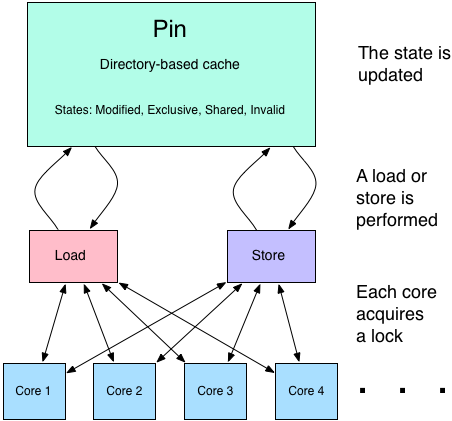
\includegraphics[scale=0.5]{images/comp_arch_sd.png}
\end{center}
\caption{System Design Diagram}
\label{sysD}
\end{figure}

\subsection{Pin-based Directory Cache Coherence}
We implemented a directory-based cache coherence protocol using Intel's Pin tool to keep track of the state of entries in an array on which load and store operations are performed.
This is shown in Figure \ref{sysD}.  
The block in green illustrates the directory-based cache implemented in pin.
The MESI protocol is illustrated in Figure \ref{MESI}.
MESI stands for ``Modified, Exclusive, Shared, Invalid" which are the names of the states assigned to an element of the array to represent the state of ownership for a given core.  
The biggest difference between this protocol and the MSI ("Modified, Shared, Invalid") protocol is that the there is an additional \emph{Exclusive} state, which means that the core has sole ownership of the data and can read or modify it at will.
The chart below illustrates the permitted states of a given element for a pair of caches:\\

\begin{center}
\begin{tabular}{|c|c|c|c|c|}
\hline
&M&E&S&I\\
\hline
M&X&X&X&\checkmark\\
E&X&X&X&\checkmark\\
S&X&X&\checkmark&\checkmark\\
I&\checkmark&\checkmark&\checkmark&\checkmark\\
\hline
\end{tabular}
\end{center}


\begin{figure}[H]
\begin{center}
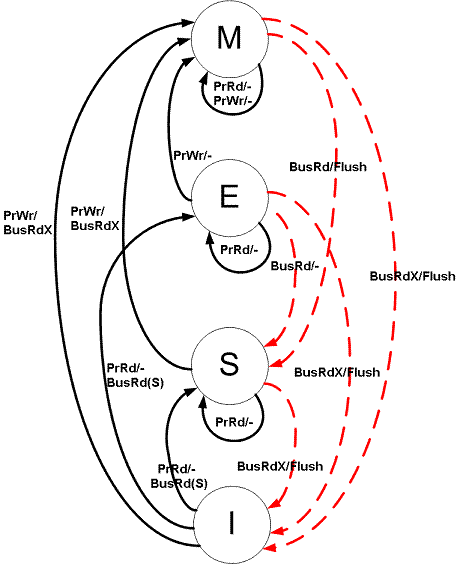
\includegraphics[scale=0.4]{images/MESI.png}
\end{center}
\caption{Illustration of the MESI protocol}
\label{MESI}
\end{figure}

\subsection{Operations}
In our system the pin tool calls a benchmark that performs load and store operations.  
The pintool monitors the state of the program and executes a special instruction when the executable performs a load or store operation.
Upon execution either of these operations, the pintool assumes control and updates the state of the directory.
Figure \ref{sd2} illustrates this transfer of control.
\begin{figure}[H]
\begin{center}
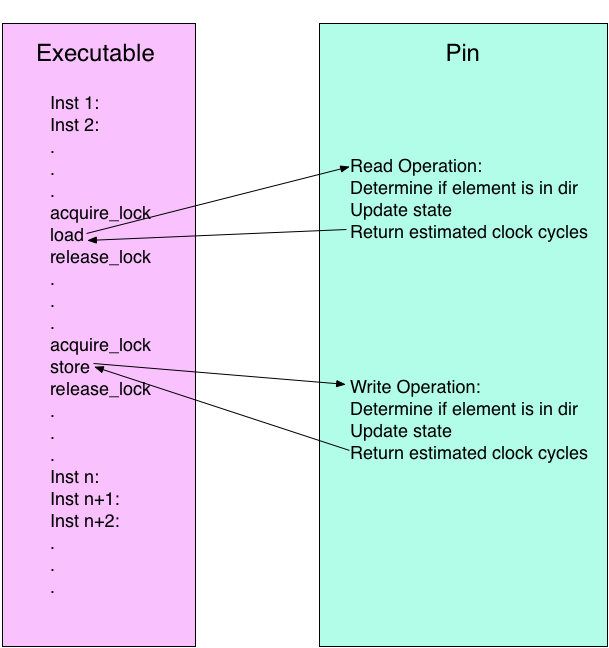
\includegraphics[scale=0.4]{images/sd2}
\end{center}
\caption{Transfer of control between the executable and pin tool}
\label{sd2}
\end{figure}

As can be seen in the diagram when the program begins executing it executes a series of instructions until it gets to a load or store function.
Prior to entering one of these functions the core must gain control of a lock.
Once it gets control of the lock, it executes the function and pin assumes control.  
Pin updates the state of the directory for the given element and estimates a number of clock cycles that the operation took to complete.
Once the executable regains control of the execution, it releases the lock and proceeds.

\subsection{Test-and-Set}
We implemented \emph{test-and-set} to compare to the \emph{pthreads} library.
Test-and-set is a series of instructions used to acuire a lock in order to perform a read or write.
The following code was used to perform the test-and-set.
\emph{lockTS} is set to 0 to release the lock.
The code was written for \emph{x86\_64}.

\begin{verbatim}
void testAndSet(int *lockTS) {
    int result = 1;
    int var2 = 0;
    asm volatile( "enter_region: lock;"
        "xchg %0, %1;"
        : "=r"(result), "=m"(*lockTS)
        : "0"(result), "m"(*lockTS)
        : "memory");
    asm volatile("cmp %%rbx, %%rax" : "=b"(result) : "b" (result), "a" (var2));
    asm volatile("jne enter_region");
}
\end{verbatim}

\subsection{Assumptions about the architecture}
In order to execute benchmarks we had to estimate the clock cycles consumed for a given operation.
Transferring a core from the \emph{Invalidate} state to \emph{Modified} state in order to perform a write requires more clock cycles than performing a write if the core already has the data in the \emph{Modified} state.
The following numbers were used in calculating the time it takes in order to perform an operation.

\begin{center}
\begin{tabular}{lc}
Time to transfer on bus & 2\\
wait time & 0\\
lookup & 5\\
flush & 7\\
\end{tabular}
\end{center}

We varied the lookup time for our experiments.  The other numbers remained constant. 
We assumed that there was no contention on the bus.
We also assumed that there was no time spent waiting.

\section{Experiments and results}\label{sec:results}
The benchmarks we used were based on the YCSB benchmarks \cite{ycsb}.
Workloads were created based on YCSB's A,B, and C workloads.
YCSB's A workload has a mix of 50/50 reads and writes.
The B workload has a 95/5 reads/writes mix.
The C workload is 100\% read.
Experiments were run to profile the efficiency of test-and-set versus the pthread library.
Table \ref{table:comp} shows the results using the above assignments for operations.

\begin{center}
\begin{table}[h]
\begin{tabular}{|ccc|} 
\hline
Workload & Pthread & Test-and-set\\
\hline
50/50 reads/writes & 703305.5 & 1978526.8\\
95/5 reads/writes & 372950.9 & 1442804.1\\
100/0 reads/writes & 461592.1 & 1488482.8\\
\hline
\end{tabular}
\caption{Table of Peformance for Pthread vs. Test-and-set}
\label{table:comp}
\end{table}
\end{center}

As can be seen in the table above the pthread library performs better than the test-and-set lock.
The reason for this increase in performance is that the test-and-set spins on the lock which wastes clock cycles.
A graph of the performance of the pthread library and test-and-set is shown in Figure \ref{pthreadvsts}

\begin{figure}[H]
\begin{center}
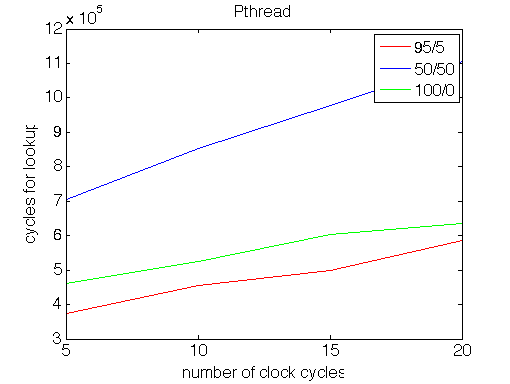
\includegraphics[scale=0.5]{images/pthread}
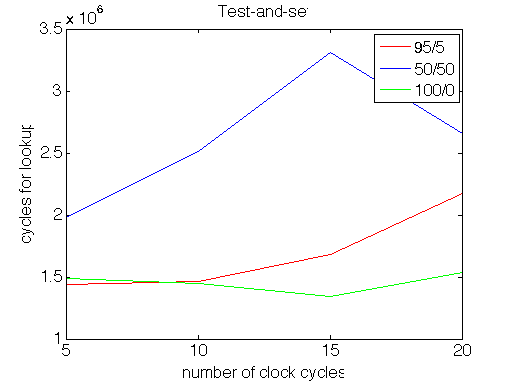
\includegraphics[scale=0.5]{images/test-and-set}
\end{center}
\caption{Transfer of control between the executable and pin tool}
\label{pthreadvsts}
\end{figure}

One key difference that can be seen in the pthread and test-and-set graphs is that the pthread graph is monotonously increasing as the number of clock cycles assigned to the Lookup operation increases.
For test-and-set the graph does not perform the same way which implies that there is an inefficiency in lock acquisition.  
The most likely cause of this is that the test-and-set function essentially uses a while loop to grab the lock and wastes clock cycles attempting to acquire it.

\section{Conclusions}\label{sec:conclusion}



\bibliographystyle{plain}
\bibliography{biblio}

\end{document}
